    \textbf{Задание №3-4.} Самостоятельно изучить нотацию IDEF1X для представления диаграммы «сущность-связь». Создать схему базы данных в нотации IDEF1X. Разработать структуру базы данных и составить описание столбцов таблиц базы данных, включающее: имя столбца, назначение (какие данные хранятся), тип данных, допускает ли столбец пустые значения. Библиотека. База данных должна содержать следующие данные: информацию об имеющихся изданиях, информацию о читателях, формуляры для каждого издания. Предусмотреть возможность анализа следующих показателей: выдать рекомендации для читателя с учетом его пола, возраста и прочитанных книг на основании общей статистики.\label{sec:3} \label{sec:4}

    \begin{figure}[H]
        \centering
        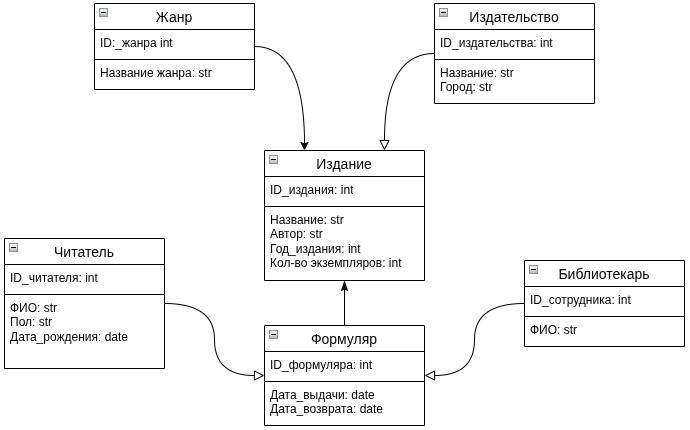
\includegraphics[width = 1 \textwidth]{picture/Class.png}
        \caption{Схема базы данных в нотации IDEF1X}
    \end{figure}
